% Copyright (c) 2015 Benito Palacios Sánchez - All Rights Reserved.
% Esta obra está licenciada bajo la Licencia Creative Commons Atribución 4.0
% Internacional. Para ver una copia de esta licencia, visita
% http://creativecommons.org/licenses/by/4.0/.

\section[Fan-traducciones]{Traducciones no oficiales}
\subsection{Saga Pokémon}
\begin{frame}{Saga Pokémon}

\begin{columns}
  \begin{column}{0.6\textwidth}
    \begin{wideitemize}
        \item Franquicia de \textit{The Pokémon Company} fundada en 1995.
        \note[item]{Se fundó en 1995 por Satoshi Tajiri cuando diseñaba muñecos para la empresa Creatures Inc.}

        \item Videojuegos desarrollados por \textit{Game Freak} para consolas de Nintendo.
        \note[item]{Exclusivos de Nintendo. A día de hoy cuenta con merchandaising, ropa, cartas, películas, anime, manga, etc.}

        \item Segunda franquicia más exitosa a nivel mundial.
        \note[item]{En 2010 se llegaron a los 200 millones de copias vendidas. Solo la marca ganó en 2014 \$2.000 millones}
    \end{wideitemize}
  \end{column}

  \begin{column}{0.4\textwidth}
    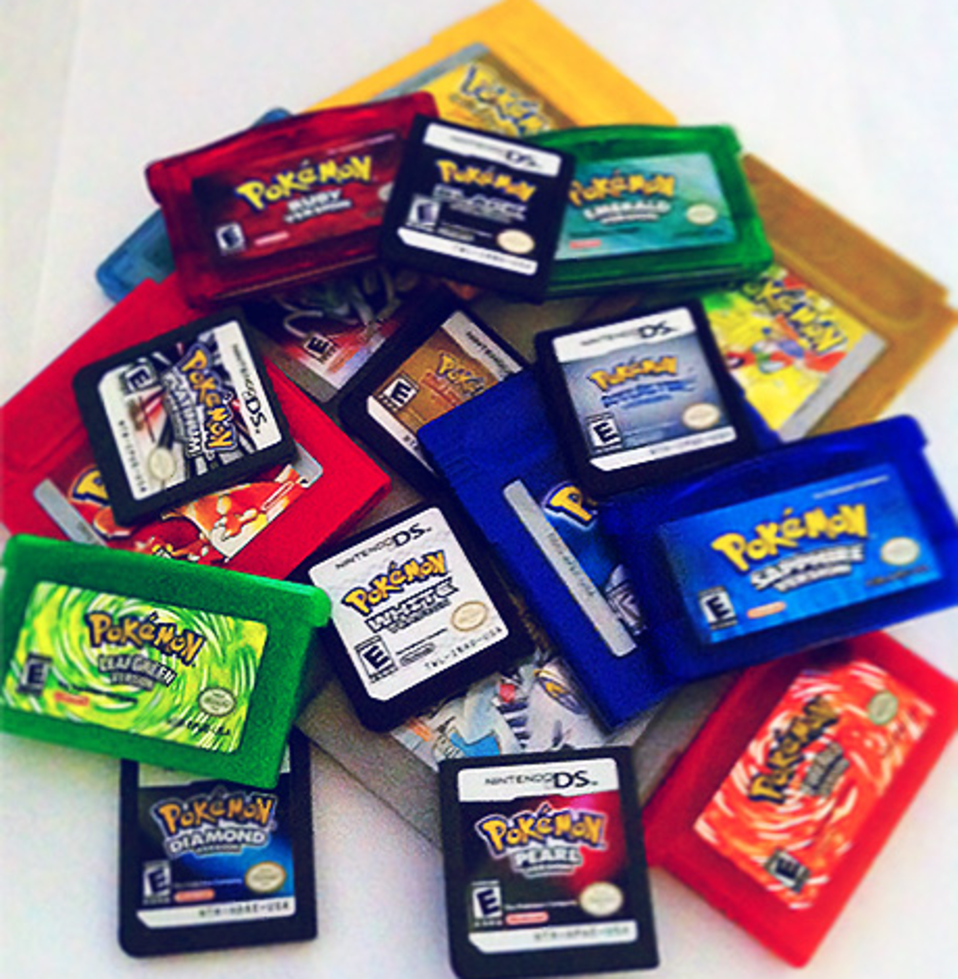
\includegraphics[width=\textwidth]{imgs/pokemon_cart.pdf}
  \end{column}
\end{columns}

\end{frame}

\begin{frame}{Metodología}
\end{frame}

\begin{frame}{Pokémon Perla y Diamante}

\end{frame}

\begin{frame}{Pokémon HeartGold y SoulSilver}

\end{frame}

\begin{frame}{Pokémon Blanco y Negro}

\end{frame}

\begin{frame}{Pokémon Conquest}

\end{frame}

\subsection{Ninokuni: El Mago de las Tinieblas}
\begin{frame}{Ninokuni: El Mago de las Tinieblas}

\end{frame}
